\documentclass[12pt, hyperref={bookmarks=false}, show notes]{beamer}
% Switch to this for handouts
%\documentclass[12pt,handout]{beamer}

% Text
	\usepackage[T1]{fontenc}
  %\usepackage{emerald}
	\usepackage[utf8]{inputenc}
	\usepackage[english]{babel}
	% \usepackage[bitstream-charter]{mathdesign} % Serif font (Charter BT).
	\usepackage[scaled=0.84]{DejaVuSansMono} % Monospaced font.
	\def\sfdefault{SourceSansPro-TLF} % Sans serif font.
	\usepackage{textcomp}

% Maths
  \usepackage{amsmath}
  \usepackage{mathtools}
  \usepackage{siunitx}

% Graphics
  \usepackage{graphicx}
  \usepackage[caption=false]{subfig}
	\usepackage{tikz}
  \usepackage{pgfplots}
  \pgfplotsset{compat=1.10}
	% ADD TIKZ LIBRARIES
  \usetikzlibrary{calc}
  \usetikzlibrary{arrows.meta}
  %\usepackage{tikz-qtree}
  \usetikzlibrary{decorations.pathmorphing}
  \usetikzlibrary{matrix,shapes,positioning,fit}
  \usepgfplotslibrary{external}
  \tikzexternalize[prefix=gfx/tikz/]
  \tikzexternaldisable % Disable by default

  \tikzstyle{bigblock} = [thick, rectangle, draw, fill=clnode, text width=4.5em, text centered, minimum height=4em]
  \tikzstyle{smallblock} = [thick, rectangle, draw, fill=clnode, text width=4.5em, text centered, minimum height=3em]
  \tikzstyle{database} = [thick, cylinder, draw, shape border rotate=90, aspect=0.15, fill=clnode, text width=3em, text centered, minimum height=4em]
  \tikzstyle{line} = [draw, -stealth, thick]
  %\tikzstyle{model} = [draw, ellipse,fill=red!20, minimum height=2em]
  \tikzstyle{container} = [rectangle, draw, inner sep=0.6 cm, dashed, fill=clshade]
  \tikzstyle{node} = [thick, circle, draw, fill=clnode, text width=1.5em, text centered, minimum height=1.5em]
  
  \usepackage{pgfgantt}
  \usepackage{mdframed}
  \newmdenv [align=center, backgroundcolor=color3!10, linecolor=color3!50, linewidth=1pt]{mtjbox}

	\usepackage{xcolor}
    \definecolor{color1}{cmyk}{100,50,0,0}   % blue
    \definecolor{color2}{cmyk}{0,80,100,0}   % vermillion
    \definecolor{color3}{cmyk}{97,0,75,0}    % blueish green
    \definecolor{color4}{RGB}{204,121,167}    % reddish purple
    \definecolor{color5}{RGB}{230,159,0}   % orange
    \definecolor{clnode}{gray}{0.85}
    \usepackage{colortbl}
% Misc
\usepackage{booktabs}
\usepackage{enumerate}
\usepackage{pdfpages}
\usepackage{pgfpages}
%\usepackage{setspace}
%\usepackage{multimedia}

% Box colors.
\definecolor{clframe}{gray}{0.75}
\definecolor{clshade}{gray}{0.95}
\definecolor{clcodeshade}{gray}{0.93}

% Code colors.
\definecolor{javared}{rgb}{0.6,0,0}            % for strings
\definecolor{javagreen}{rgb}{0.25,0.5,0.35}    % comments
\definecolor{javapurple}{rgb}{0.6,0,0.5}       % keywords
\definecolor{javadocblue}{rgb}{0.25,0.35,0.75} % javadoc

%More colors
\definecolor{colorA}{HTML}{5DA5DA} % blue
\definecolor{colorB}{HTML}{FAA43A} % orange
\definecolor{colorC}{HTML}{60BD68} % green
\definecolor{colorD}{HTML}{F17CB0} % pink
\definecolor{colorE}{HTML}{B2912F} % brown
\definecolor{colorF}{HTML}{B276B2} % purple
\definecolor{colorG}{HTML}{DECF3F} % yellow
\definecolor{colorH}{HTML}{F15854} % red
\definecolor{colorI}{HTML}{4D4D4D} % gray

\colorlet{colorAshade}{colorA!80!black}
\colorlet{colorBshade}{colorB!80!black}
\colorlet{colorCshade}{colorC!80!black}
\colorlet{colorDshade}{colorD!80!black}
\colorlet{colorEshade}{colorE!80!black}
\colorlet{colorFshade}{colorF!80!black}
\colorlet{colorGshade}{colorG!80!black}
\colorlet{colorHshade}{colorH!80!black}
\colorlet{colorIshade}{colorI!80!black}

\usepackage{listings}

\lstdefinestyle{javastyle}{%
  language=Java,
  keywordstyle=\color{javapurple}\bfseries,
  stringstyle=\color{javared},
  commentstyle=\color{javagreen},
  morecomment=[s][\color{javadocblue}]{/**}{*/}
}

\lstnewenvironment{javacode}[1][]{%
  \lstset{style=javastyle, #1}
}{}

\lstset{
  columns=flexible,
  escapechar=",
  escapeinside={(*@}{@*)},
  basicstyle=\ttfamily\footnotesize,
  frame=single, backgroundcolor=\color{clshade}, rulecolor=\color{clframe},
  framerule=\fboxrule, xleftmargin=3.4pt, xrightmargin=3.4pt, belowskip=\smallskipamount,
  captionpos=b,
  numbers=left,
  numberstyle=\scriptsize,
  numbersep=7pt,
  tabsize=2,
  keepspaces=true,
  showspaces=false,
  showstringspaces=false,
  breaklines=true,
  breakatwhitespace=true,
  postbreak=\raisebox{0ex}[0ex][0ex]{\ensuremath{\color{red}\hookrightarrow\space}}
}



\setbeamertemplate{navigation symbols}{}
%\setbeamertemplate{bibliography item}[text]

%\usepackage{caption}
\usetheme{/amsterdam}
\date{June 15, 2015}

%Uncomment for handouts: (remember to uncomment in line 1+2, too)
%\usepackage{beamertheme/handoutWithNotes}
%\pgfpagesuselayout{4 on 1 with notes}[a4paper,border shrink=5mm]

% Comment for handouts or slides without notes:
\setbeameroption{show notes on second screen=right}
\setbeamertemplate{note page}{%
  \insertnote%
}

% Table of content dybde (0-index)
%\setcounter{tocdepth}{1}

% BibLaTeX
%\usepackage{csquotes}
%\usepackage[
%backend=bibtex,
%citestyle=numeric,
%bibstyle=numeric,
%maxcitenames=3,
%maxbibnames=99,
%url=true]{biblatex}
%\addbibresource{../rapport/references/refs.bib}
%\addbibresource{extrasources.bib}
%\usepackage{../style/biblatex_custom_formatting}

\graphicspath{{gfx/}{../report/graphics/}{../report/graphics/tikz}}

\begin{document}

%\captionsetup[figure]{font=small,singlelinecheck=off,justification=raggedright}

\title[Improving Wikipedia Linking: A Feature Learning Approach]{Improving Wikipedia Linking: A Feature Learning Approach}
% \author[\insertframenumber /\inserttotalframenumber]{sw609f15}
\makeatletter
  \defbeamertemplate*{footline}{myminiframes theme}
  {%
    \begin{beamercolorbox}[colsep=1.5pt]{upper separation line foot}
    \end{beamercolorbox}
    \hbox{%
      \begin{beamercolorbox}[wd=.75\paperwidth,ht=2.5ex,dp=1.125ex,%
        leftskip=.3cm,rightskip=.3cm plus1fil]{title in head/foot}%
        \leavevmode{\usebeamerfont{title in head/foot}\insertshorttitle}%
      \end{beamercolorbox}%
      \begin{beamercolorbox}[wd=.15\paperwidth,ht=2.5ex,dp=1.125ex,%
        leftskip=.3cm,rightskip=.3cm]{title in head/foot}%
        {\usebeamerfont{author in head/foot}\usebeamercolor[fg]{author in head/foot}\insertshortauthor}
      \end{beamercolorbox}%
      \begin{beamercolorbox}[wd=.1\paperwidth,ht=2.5ex,dp=1.125ex,%
        leftskip=.3cm,rightskip=.3cm,center]{title in head/foot}%
        {\usebeamerfont{author in head/foot}\usebeamercolor[fg]{author in head/foot}\insertframenumber/\inserttotalframenumber}%
      \end{beamercolorbox}%
    }%
    \begin{beamercolorbox}[colsep=1.5pt]{lower separation line foot}
    \end{beamercolorbox}
  }
\makeatother

% Adding front slide.
{
\setbeamercolor{background canvas}{bg=}

\includepdf[pages=1]{frontslide.pdf}
}
\note{
    Noter, noter, noter!
}

\begin{frame}
  \frametitle{Contents}
  \tableofcontents
  \note{
  \begin{itemize}
    \item Notes
    \item notes
    \item notes..
  \end{itemize}
}
\end{frame}


\chapter{Introduction}
\dummy

\section{Bootstrapping the Project}
\dummy

\section{Project Goals}
\dummy

\section{Report Organization}
\dummy
\section[Design 1]{Design 1}
% Første parameter i [] er tekst i header. {} er i indholdsfortegnelsen.

% Slide med emneoverskrift.
\begin{frame}
  \frametitle{}
  \begin{center}
    {\Huge System Design 1}
  \end{center}
\end{frame}
\note{
  \begin{itemize}
		\item Notes...
  \end{itemize}
}

% Normal slide:
\begin{frame}
    \frametitle{System Design 1}
    \centering
    \begin{itemize}
      \item System characteristics \& requirements
      \item Design goals
      \item Architecture
    \end{itemize}
\end{frame}

\begin{frame}
    \frametitle{System characteristics \& requirements}
    \centering
    \begin{itemize}
      \item Data processing - backend
      \begin{itemize}
        \item Maintainable
        \item Scalable
      \end{itemize}
      \item Presentation to users - frontend
      \begin{itemize}
        \item Fast response times
      \end{itemize}
    \end{itemize}
\end{frame}
\note{
  \begin{itemize}
		\item We chose machine learning approach - Data processing by nature
    \item Calculation heavy - backend
    \item Maintainable - experimentation + prototyping
    \item Scalable - work with larger datasets
  \end{itemize}
}

\begin{frame}
    \frametitle{Design goals}
    \centering
    \begin{itemize}
      \item Modularity
      \begin{itemize}
        \item Separated components
        \item Data protocol - loose coupling
        \item Individual component evolution
      \end{itemize}
      \item Scalability
      \begin{itemize}
        \item Distributed components - horizontal scaling
        \item Solve bottlenecks as they happen
        \item TODO: De komponenter der ikke kan scales horisontalt - nævn hvilke, kan scales vertikalt individuelt
        \item Offloading
      \end{itemize}
    \end{itemize}
\end{frame}
\note{
  \begin{itemize}
		\item Individual component evolution - languages and platforms
  \end{itemize}
}

\begin{frame}
    \centering
    \resizebox{\textwidth}{!}{%
      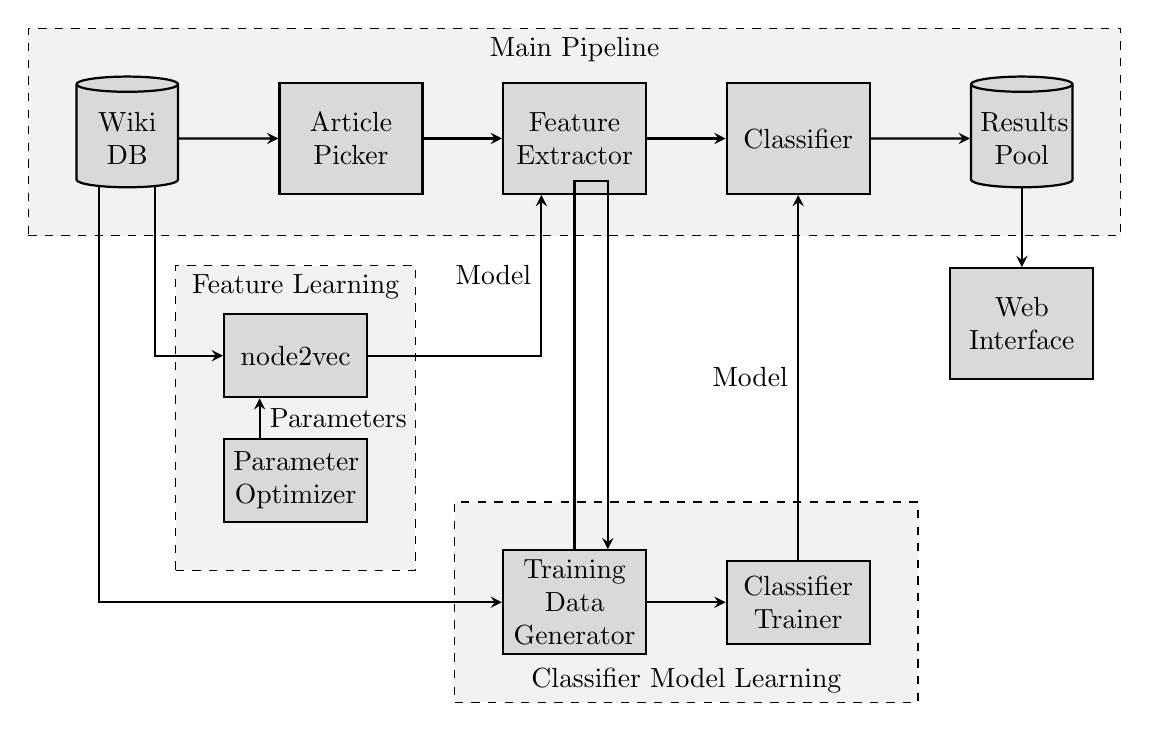
\begin{tikzpicture}[node distance = 2.84cm, auto]
    \node [database, yshift=1em] (db) {Wiki DB};
    \node [bigblock, right of=db] (ap) {Article Picker};
    \node [bigblock, right of=ap] (tfl) {Feature Extractor};
    \node [bigblock, right of=tfl] (classifier) {Classifier};
    \node [database, right of=classifier] (db2) {Results Pool};
    \node [bigblock, below=1cm of db2] (web) {Web Interface};
    
    %\node [above=1cm of ap] (inputarticle) {};
    
    \node [smallblock, below=1.5cm of ap, xshift=-2em] (n2v) {node2vec};
    \node [smallblock, below=.5cm of n2v] (paropt) {Parameter Optimizer};
    
    \node [smallblock, below=4.5cm of tfl] (prepper) {Training Data Generator};
    \node [smallblock, right of=prepper] (classifierTrainer) {Classifier Trainer};
    
    \begin{scope}[on background layer]
    \node [container, fit=(n2v)(paropt)] (container1) {};
    \node[below] at (container1.north) {Feature Learning};
    \node [container, fit=(prepper)(classifierTrainer)] (container2) {};
    \node[above] at (container2.south) {Classifier Model Learning};
    
    \node [container, fit=(db)(db2)] (container3) {};
    \node[below] at (container3.north) {Main Pipeline};
    \end{scope}
    
    %\draw [->] (db) -- (n2v);
    
    \path [line] (db) -- (ap);
    %\path [line] (inputarticle) -- (ap);
    \path [line] (ap) -- (tfl);
    \path [line] (tfl) -- (classifier);
    \path [line] (classifier) -- (db2);
    \path [line] (db2) -- (web);
    
    \path [line] (db.300) |- (n2v);
    %\path [line] (db.300) |- (paropt);
    \path [line] (db.240) |- (prepper);
    
    \path [line, swap, transform canvas={xshift=-1.3em}] (paropt) -- node{Parameters} (n2v);
    \path [line] (n2v.east) -| node [near end] {Model} ([xshift=-1.2em]tfl.south);
    
    \path [line] (prepper) -- (classifierTrainer);
    %\path [line] (prepper) -- (tfl);
    %\path [line] ([xshift=1.2em]tfl.south) -- ([xshift=1.2em]prepper.north);
    \draw [line] (prepper.north) |- ([xshift=1.2em, yshift=0.5em]tfl.south) -- ([xshift=1.2em]prepper.north);
    
    \path [line] (classifierTrainer) -- node{Model} (classifier);
    
  \end{tikzpicture}
    }
\end{frame}
\section[Wronglywent]{What Went Wrong?}
% Første parameter i [] er tekst i header. {} er i indholdsfortegnelsen.

% Slide med emneoverskrift.
\begin{frame}
  \frametitle{}
  \begin{center}
    {\Huge What Went Wrong?}
  \end{center}
\end{frame}
\note{
  \begin{itemize}
		\item Notes...
  \end{itemize}
}

% Normal slide:
\begin{frame}
    \frametitle{Some Example Title}
    \framesubtitle{Some example subtitle}
    \centering
    Some text, content, etc.
\end{frame}
\note{
	\begin{itemize}
    \item Notes here...
	\end{itemize}
}
\section[UI]{User Interface}
% Første parameter i [] er tekst i header. {} er i indholdsfortegnelsen.

% Slide med emneoverskrift.
\begin{frame}
  \frametitle{}
  \begin{center}
    {\Huge User Interface}
  \end{center}
\end{frame}
\note{
  \begin{itemize}
		\item Introduce
    \item Design choices
    \item Testing
    \item Demo
  \end{itemize}
}

\begin{frame}
    \frametitle{The Design Process}
    \framesubtitle{Starting the process}
    \begin{itemize}
    	\item Design from requirements
    	\item Incremental development
    \end{itemize}
\end{frame}
\note{
	\begin{itemize}
    \item Use Web Engneering Techniques.
    \item built on requirement engineering.
    \item Little by Little.
    \item Fit well with project.
	\end{itemize}
}

\begin{frame}
    \frametitle{The Design Process}
    \framesubtitle{Gathering requirements}
    \begin{itemize}
    	\item Information Flow Diagram
    \end{itemize}
    \includegraphics[width=\textwidth]{wikiAPI.pdf}
\end{frame}
\note{
	\begin{itemize}
    \item Organizational Concerns.
    \item Information Delivery.
    \item Understanding our model wishes.
    \item Diagram
    \item Incremental -> simple editors
    \item Created two requirements
	\end{itemize}
}

\begin{frame}
    \frametitle{The Design Process}
    \framesubtitle{Gathering Requirements}
    \begin{itemize}
    	\item A user must be able to query the UI for link suggestions.
    	\item A user should be able to submit reviews of link suggestions.
    \end{itemize}
\end{frame}
\note{
	\begin{itemize}
    \item First and foremost
    \item Secondly -> reaction
    \item learn from it.
	\end{itemize}
}

\begin{frame}
    \frametitle{The Design Process}
    \framesubtitle{Creating a Solution}
    \begin{itemize}
    	\item User Demographic    
    	\item API > GUI
    \end{itemize}
\end{frame}
\note{
	\begin{itemize}
    \item Create Solution Idea
    \item STEP1: Analyze TARGET
    \item Speculation NO CONTACT
    \item Bacbone -> influence
    \item ----------
    \item Reasearch -> API
    \item access as possible
    \item direct GUI
    \item API = Broad dev
    \item realistic
    \item no initiation?
	\end{itemize}
}

\begin{frame}
    \frametitle{Testing the API}
    \framesubtitle{}
    \begin{itemize}
    	\item Unit testing
    	\item Acceptance test
    \end{itemize}
\end{frame}
\note{
	\begin{itemize}
    \item integrity
    \item Django helps
    \item Presedence
	\end{itemize}
}

\begin{frame}
  \frametitle{}
  \begin{center}
    {\Huge DEMO}
  \end{center}
\end{frame}
\note{
  \begin{itemize}
		\item Notes...
  \end{itemize}
}

% \begin{frame}
%     \frametitle{Some Example Title}
%     \framesubtitle{Some example subtitle}
%     \centering
%     Some text, content, etc.
% \end{frame}
% \note{
% 	\begin{itemize}
%     \item Notes here...
% 	\end{itemize}
% }
\section[MI Test]{MI Test}
% Første parameter i [] er tekst i header. {} er i indholdsfortegnelsen.

% Slide med emneoverskrift.
\begin{frame}
  \frametitle{}
  \begin{center}
    {\Huge MI Test}
  \end{center}
\end{frame}
\note{
  \begin{itemize}
		\item Notes...
  \end{itemize}
}

% Normal slide:
\begin{frame}
    \frametitle{Some Example Title}
    \framesubtitle{Some example subtitle}
    \centering
    Some text, content, etc.
\end{frame}
\note{
	\begin{itemize}
    \item Notes here...
	\end{itemize}
}
\section[Dev. Method]{Development Method}
% Første parameter i [] er tekst i header. {} er i indholdsfortegnelsen.

% Slide med emneoverskrift.
\begin{frame}
  \frametitle{}
  \begin{center}
    {\Huge Development Method}
  \end{center}
\end{frame}
\note{
  \begin{itemize}
		\item 1) dev. method
		\item 2) then reflect upon the project
		\item 3) before conluding
		
		\item We needed to agree on dev. method.
  \end{itemize}
}

% Normal slide:
\begin{frame}
    \frametitle{Development Method}
    %\framesubtitle{Development Method}
    \begin{itemize}
			\item Choice of Paradigm
		  \begin{itemize}
				\item Traditional, analysis-heavy
				\item Agile
				\begin{itemize}
					\item Structure and practices
				\end{itemize}
			\end{itemize}
			\item Our method
			\begin{itemize}
				\item Self-organized
				\item Responding to change > following a plan
				\item Paper cards and daily status meeting
			\end{itemize}
		\end{itemize}
\end{frame}
\note{
	\begin{itemize}
		\item We \textbf{argue}... benefit from \textbf{experimental approach} (dismiss)
		\item Considered \textbf{agile approaches}
		\begin{itemize}
			\item large \textbf{emph on customer}. We have no customer.
			\begin{itemize}
				\item Easily make up and play cust. role, just for sake of fulfil. dev. met.
			\end{itemize}
			\item \textbf{emph on software/code} > documentation
			\begin{itemize}
				\item we have report
			\end{itemize}
			\item Might bring structure \& practices
			\begin{itemize}
				\item we believe we \textbf{worked suff.} to use in \textbf{ad-hoc manner}.
			\end{itemize}
		\end{itemize}
		\item Because of the \textbf{experimental nature}, decided on method that allowed this. It is Self-organized \textrightarrow{} \textbf{keeping themselv. active.}
		\begin{itemize}
			\item Mitigated by our method \textbf{open to responding to change} over following a plan.
			\item Changes happening often \textrightarrow{} yield new areas to explore
		\end{itemize}
		\item To \textbf{facilitate} our work
		\begin{itemize}
			\item immediate tasks on paper cards, \textbf{laid them visible}
			\item status meetings, \textbf{morning discuss and todo}
		\end{itemize}
	\end{itemize}
}

\section[Reflection]{Reflection}

% Slide med emneoverskrift.
%\begin{frame}
  %\frametitle{}
  %\begin{center}
    %{\Huge Reflection}
  %\end{center}
%\end{frame}
%\note{
  %\begin{itemize}
		%\item Notes...
  %\end{itemize}
%}

% Normal slide:
\begin{frame}
    \frametitle{Reflection}
    \framesubtitle{Development Method}
    \begin{itemize}
			\item Handling data\ \ >\ \ code
			\item Completed a large body of work
			\item Timeboxing status meetings
		\end{itemize}
\end{frame}
\note{
	\begin{itemize}
    \item In the large, \textbf{adequate method}
			\begin{itemize}
				\item \textbf{In part due} to experimental nature
				\item and \textbf{less emphasis} on ``lots of code''
				\item Large part was setting up tools, preparing data
			\end{itemize}
			\item Our method, being self-organized, required \textbf{discipline}
			\begin{itemize}
				\item But driven by an \textbf{interest}, we completed a large body of work
				\item Not all work is \textbf{visible} in the report
				\item because experi. nature lead to \textbf{areas with unsatis. results}.
				\item needed to backtrack from
			\end{itemize}
			\item In hindsight, \textbf{status meetings} might benefit \textbf{timeboxed}
			\begin{itemize}
				\item greater \textbf{distinction} between info. for everybody and individuals.
				\item However, led to important discussions. Necessary to disc.
			\end{itemize}

	\end{itemize}
}

\begin{frame}
    \frametitle{Reflection}
    \begin{itemize}
			\item Difficulty choosing and defining problem
			\item No prior project experience in MI area
			\item Feature Engineering \textrightarrow{} Feature Learning
		\end{itemize}
\end{frame}
\note{
	\begin{itemize}
    \item We initially \textbf{spent long time on identifying project}
		\begin{itemize}
			\item not want \textbf{trivial} project
			\item We chose project \textbf{large span} in terms of work + poss solu.
		\end{itemize}
		\item Furthermore, we have \textbf{not previously worked} on sem. proj. \textbf{of this kind}
		\begin{itemize}
			\item MI in the \textbf{area of large}/unstructured dataset, new to us
			\item Probably \textbf{underestimated, time} preparing so much data
			\item We had \textbf{difficulties defining} our project, bc. \textbf{lack of prior exp}... therefore approach experi.
			\item This caused us spend time on experiments that \textbf{not move proj. forward}... However, valuable learning experience
		\end{itemize}
		\item Experienced with feat. engi. \textbf{in beginning. 1 month}
		\begin{itemize}
			\item Realizing \textbf{not satisfying} solution, time \textbf{not properly invested}. 
		\end{itemize}
		\item \textbf{Best feature} we engineered \textrightarrow{} based on structure
		\begin{itemize}
			\item therefore a \textbf{feat.lear. approach} based on struct \textrightarrow{} good
			\item this is why we changed our \textbf{focus}
		\end{itemize}
	\end{itemize}
}

\begin{frame}
    \frametitle{What Have We Learned?}
    \begin{itemize}
			\item Take on manageable projects
			\item Feature engineering is hard
			\item Feature learning is not ``plug and play''
			\begin{itemize}
				\item Not entirely automated
			\end{itemize}
			\item Important to verify subresults in pipeline
			\begin{itemize}
				\item Careful about details and refinement of testing
			\end{itemize}
			\item Long turn-around time in timeboxed project period
		\end{itemize}
\end{frame}
\note{
	\begin{itemize}
    \item Manageable projects
		\begin{itemize}
			\item our was not manageable in beginning \textrightarrow{} \textbf{risk taking on}
			\item Demanding work, and we \textbf{pursued ideas} turned out \textbf{not satis}.
			\item However, learned a lot
		\end{itemize}
		\item for example, feature eng is hard
		\item Plug and Play: Sounded like automated process, but took longer time
		\begin{itemize}
			\item you \textbf{gain time} from not engineering, but takes time to setup
		\end{itemize}
		\item Verify results: \textbf{decrease risk of bad choices down-stream}
		\begin{itemize}
			\item This means... Careful about details and... \textbf{in isolation}
		\end{itemize}
		\item Combination of working with lots of data + timeb. proj. period.\begin{itemize}
			\item \textbf{requires thought} \textrightarrow{} factor in data is \textbf{time-consuming}.
		\end{itemize}
	\end{itemize}
}

\section[Conclusion]{Conclusion}

\begin{frame}
    \frametitle{Conclusion}
		%"How can a software solution be developed that supports Wikipedia editors by suggesting potential article links using machine learning on a graph structure?"
		\begin{itemize}
			\item System did not generalize well
			\item We re-did parts
			\begin{itemize}
				\item More promising results!
			\end{itemize}
			\item Semantic analysis?
		\end{itemize}
    
\end{frame}
\note{
	\begin{itemize}
    \item Overall, we designed and impl. software solution to suggest article links. Predictions made on structural info.
		\item Our results showed approach Did not \textbf{generalize well}
		\item However, re-did parts after turning in
		\begin{itemize}
			\item More promising results.
			\item While \textbf{not perfect}, results may \textbf{indicate} it is \textbf{possible} to predict links based on structure
			\item we believe, \textbf{further refinement} may make adequate solution
		\end{itemize}
		\item Also possible to \textbf{combine with content info} (semantic anal.)
		\item \ \ \ this may further improve results
		\item So while many things \textbf{could be done to improve} results, the \textbf{basis} for predicting links is \textbf{covered and working}, and we are \textbf{satisfied with the new results}.
	\end{itemize}
}

\section*{}

\begin{frame}
  \frametitle{Overview}
  \tableofcontents
\end{frame}

\end{document}
